\documentclass{beamer}
\usetheme{Montpellier}

\usepackage{color}
\usepackage{amsfonts}
\usepackage{comment}

%%% Al parecer necesito esto en ubuntu para los acentos
\usepackage[spanish]{babel}
\selectlanguage{spanish}
\usepackage[utf8]{inputenc}

\definecolor{myblue}{rgb}{0.25, 0, 0.75}
\definecolor{mygold}{rgb}{1,0.8,0.2}
\definecolor{gray}{rgb}{0.5, 0.5, 0.5}
\definecolor{lucia}{rgb}{0.8,0.4,0.7} 

\newcommand{\myurl}[1]{\href{http://#1}{\textcolor{gray}{\texttt{#1}}}}
\newcommand{\myem}[1]{\structure{#1}}
\newcommand{\myurlshort}[2]{\href{http://#1}{\textcolor{gray}{\textsf{#2}}}}

\newcommand{\RPackage}[1]{\textcolor{gray}{\textsf{#1}}}
\newcommand{\pl}[1]{\texttt{#1}}
\newcommand{\RCode}[1]{\texttt{#1}}
\newcommand{\RFunction}[1]{\textsf{#1}}
\newcommand{\RClass}[1]{\textcolor{mygold}{\textsf{#1}}}
\newcommand{\BIOCfunction}[1]{\textcolor{orange}{#1}}

\setbeamercolor{example text}{fg=lucia}
\setbeamertemplate{sections/subsections in toc}[ball unumbered]
\setbeamertemplate{frametitle continuation}[from second][]
\setbeamertemplate{itemize subitem}[triangle]
\setbeamertemplate{footline}[page number]
\setbeamertemplate{caption}[numbered]
\setbeamertemplate{navigation symbols}{}

\renewcommand{\footnotesize}{\fontsize{6.10}{12}\selectfont}

\def\argmax{\operatornamewithlimits{arg\,max}}
\def\argmin{\operatornamewithlimits{arg\,min}}

%%\bibliographystyle{plain}


\title{Seminario III: R/Bioconductor}
\author{Leonardo Collado Torres \\ lcollado@lcg.unam.mx \\  Licenciado en Ciencias Genómicas \\ \myurl{www.lcg.unam.mx/\string~lcollado/}}
\date{
Agosto - Diciembre, 2009
}








\usepackage{Sweave}
\begin{document}

\begin{frame}[allowframebreaks]
  \titlepage
\end{frame}

\section*{Visi\'on General de la clase}

\begin{frame}[allowframebreaks]
  \frametitle{Cómo usar \pl{R}}
  \tableofcontents[hideallsubsections]
\end{frame}

%%%%%%%%%%%%%%%%%%%%%%%%%%%%%%%%%%%%%%%%%%%%%%%%%%%%%%%%%%%%%%%%%%%%%%%%%%%
\section{Bienvenida}

\begin{frame}[allowframebreaks]
  \frametitle{Y as\'i comienza}
  \begin{itemize}
  \item Primer curso exclusivo de Bioconductor de 32 horas en la LCG
  \item Inspirado en el BioC2009
  \item Todo el material esta disponible en ingl\'es y español
  \item Clases en Ingl\'es: \myurlshort{bioconductor.org/workshops/}{Bioc} y \myurlshort{ocw.mit.edu/OcwWeb/web/home/home/index.htm}{OCW}
  \item Asistentes Alejandro, Jos\'e y V\'ictor
  \item P\'agina oficial del curso: \url{http://www.lcg.unam.mx/~lcollado/B/}
  \item Recuerden utilizar el foro para aclarar sus dudas
  \end{itemize}
\end{frame}

\begin{frame}[allowframebreaks]
  \frametitle{Programa}
  \begin{itemize}
  \item Objetivos
  \item Proyecto: Buscar artículos de Bioconductor
  \item Una clase de muestra
  \item Evaluaci\'on
  \item Calendario de clases \emph{tentativo}
  \end{itemize}
\end{frame}

\begin{frame}[allowframebreaks]
  \frametitle{Informaci\'on del curso}
  \begin{itemize}
  \item El curso es proporciona una visi\'on general del curso.
  \item Algunos expertos en Bioconductor hicieron comentarios acerca del curso!
  \item El calendario guarda una estrecha relaci\'on con \emph{Bioinform\'atica y Estad\'istica I}. Como es el caso de \pl{Biostrings}.
  \item Buscamos que un experto nos visite :)
  \end{itemize}
\end{frame}


\begin{frame}[allowframebreaks]
  \frametitle{Grabaci\'on de videos}
  \begin{itemize}
  \item Este es el curso piloto de la LCG para el OpenCourseWare
  \item Todas las clases ser\'an videograbadas!
  \item As\'i que \alert{Ingl\'es} todo el tiempo
  \item Hay un retraso de una semana
  \end{itemize}
\end{frame}

%%%%%%%%%%%%%%%%%%%%%%%%%%%%%%%%%%%%%%%%%%%%%%%%%%%%%%%%%%%%%%%%%%%%%%%%%%%
\section{Introducci\'on b\'asica a  \pl{R}}

\begin{frame}[allowframebreaks]
  \frametitle{Antecedentes de \pl{R}}
  \begin{itemize}
  \item \pl{R} es una implementaci\'on open-source del lenguaje S: Becker, Wilks y Chambers. \pl{S-PLUS} es una de uso privado.
  \item Creado por Ross Ihaka y Robert Gentleman\footnote{El tambi\'en cre\'o el proyecto de Bioconductor}
  \item Es un lenguaje interpretado y \alert{\emph{vive}} en el momento de interpretaci\'on.
  \item Es muy \'util como ambiente de programaci\'on: gr\'aficas, estad\'isticas, paquetes biol\'ogicos (gen\'omicos) como los de Bioconductor.
  \item Ciclo de lanzamientos de seis meses. Versiones estables y de desarrollo. 
  \item \pl{R} es un lenguaje multi plataforma: Windows, Linux/Unix y Mac.
  \item R Core y la Comprehensive R Archive Network (CRAN) \url{http://cran.r-project.org}
  \end{itemize}
\end{frame}

\begin{frame}[allowframebreaks]
  \frametitle{Instalando \pl{R}}
  \begin{itemize}
  \item Para \BIOCfunction{Windows} y \BIOCfunction{Mac}, descarga el binario de CRAN, doble click y a seguir las instrucciones.
  \begin{itemize}
  \item Lanzamientos \myurlshort{cran.r-project.org/bin/windows/base/}{estables en Windows} y \myurlshort{cran.r-project.org/bin/macosx/}{Estables en Mac}.
  \end{itemize}
  \item Para \BIOCfunction{Linux/Unix}, depender\'a del sabor de tu preferencia. Suponiendo que tienes Ubuntu, entonces sigue \myurlshort{cran.r-project.org/bin/linux/ubuntu/}{estas instrucciones} para obtener la versi\'on estable m\'as reciente, pues \pl{sudo apt-get install r-base} usualmente no est\'a actualizado para la versi\'on m\'as reciente.
  \item Para este curso necesitar\'an la versi\'on de desarrollo de \pl{R} develllamada 2.10.0devel y Bioconductor versi\'on 2.5.
  \begin{itemize}
  \item Ya est\'a instalado en Montealban (Windows) y pronto estar\'a en los servidores Solaris.
  \end{itemize}
  \end{itemize}
\end{frame}

\begin{frame}[allowframebreaks, fragile]
  \frametitle{Una sesi\'on b\'asica de \pl{R}}
  \begin{itemize}
  \item Se recomienda el uso de  \BIOCfunction{Emacs} o \BIOCfunction{XEmacs} para trabajar con \pl{R}. En el \'ultimo de los casos usa un editor de textos, copia y pega tus comandos \footnote{En Windows pueden usar la interfaz gr\'afica de R y correr sus comandos con \pl{CTRL + R}.}.
  \item Teclea \pl{R} en tu terminal o haz doble click en el \'icono de \pl{R}. Se muestra alguna informaci\'on b\'asica.
  \item Se puede usar \pl{R} simplemente como una calculadora, as\'i que escribe algunos comandos :)  
\begin{Schunk}
\begin{Sinput}
> 2 + 3 * 5
\end{Sinput}
\begin{Soutput}
[1] 17
\end{Soutput}
\begin{Sinput}
> 2^3
\end{Sinput}
\begin{Soutput}
[1] 8
\end{Soutput}
\begin{Sinput}
> 6/3
\end{Sinput}
\begin{Soutput}
[1] 2
\end{Soutput}
\begin{Sinput}
> sqrt(pi)
\end{Sinput}
\begin{Soutput}
[1] 1.772454
\end{Soutput}
\begin{Sinput}
> exp(log(5))
\end{Sinput}
\begin{Soutput}
[1] 5
\end{Soutput}
\end{Schunk}
  \item Se pueden insertar comentarios en el c\'odigo con el s\'imbolo de  \#.
  \item Sal usando las funciones \BIOCfunction{q} o \pl{quit}.
\begin{Schunk}
\begin{Sinput}
> q("no")
\end{Sinput}
\end{Schunk}
  \end{itemize}
\end{frame}

\begin{frame}[allowframebreaks, fragile]
  \frametitle{Espacio de trabajo e historial}
  En algunas ocasiones es necesario interrumpir tu trabajo as\'i que guardar tus objetos de \pl{R}, historial o sesi\'on es muy \'util.
  \begin{itemize}
  \item Es posible \BIOCfunction{salvar} y \BIOCfunction{cargar} objetos especificando los objetos, su ruta y el nombre de archivo en un archivo \alert{.Rda}.
\begin{Schunk}
\begin{Sinput}
> save(object1, object2, file = file.path("folder", 
+     "file.Rda"))
> load(file = file.path("folder", 
+     "file.Rda"))
\end{Sinput}
\end{Schunk}
  \item Para ver tus comandos recientes usa la funci\'on \BIOCfunction{history}. Puedes salvar y guardar tu historial usando los comandos \BIOCfunction{savehistory} y \BIOCfunction{loadhistory}.
\begin{Schunk}
\begin{Sinput}
> history()
> savehistory(file = file.path("folder", 
+     "file.Rhistory"))
> loadhistory(file = file.path("folder", 
+     "file.Rhistory"))
\end{Sinput}
\end{Schunk}
  \item Puedes guardar tu sesi\'on en un archivo\pl{.Rdata} mediante la especificaci\'on de ello al momento de salir o con la funci\'on \BIOCfunction{save.image} y usando \BIOCfunction{load} para cargarla de nuevo.
\begin{Schunk}
\begin{Sinput}
> q(save = "yes")
> save.image(file = file.path("folder", 
+     "file.Rdata"))
> load(file = file.path("folder", 
+     "file.Rdata"))
\end{Sinput}
\end{Schunk}
  \item Mientras trabajas, a veces ser\'a necesario cambiar el directorio en donde te encuentras o ver lo que est\' ah\'i contenido. Funciones como \BIOCfunction{getwd}, \BIOCfunction{setwd}, \BIOCfunction{list.files()} y \BIOCfunction{dir()} ser\'an \'utiles.
  \end{itemize}
\end{frame}

%%%%%%%%%%%%%%%%%%%%%%%%%%%%%%%%%%%%%%%%%%%%%%%%%%%%%%%%%%%%%%%%%%%%%%%%%%%
\section{Buscando ayuda}

\begin{frame}[allowframebreaks, fragile]
  \frametitle{Ayuda en \pl{R}}
  Hay muchas formas de obtener ayuda en \pl{R}. Se mencionan algunas a continuaci\'on.
  \begin{itemize}
  \item La funci\'on m\'as b\'asica para buscar ayuda es, \BIOCfunction{help}. Esta es una forma m\'as corta: \BIOCfunction{?}
\begin{Schunk}
\begin{Sinput}
> help(quit)
> `?`(q)
\end{Sinput}
\end{Schunk}
  \item Una buena herramienta es el buscador de ayuda que se acciona mediante la funci\'on \BIOCfunction{help.start}.Durante la sesi\'on, las p\'aginas de ayuda se abrir\'an en tu navegador.
\begin{Schunk}
\begin{Sinput}
> help.start()
\end{Sinput}
\end{Schunk}
  \item Otras funciones que se usan frecuentemente son \BIOCfunction{apropos} y \BIOCfunction{args}. La primera enlista todas las funciones cuyo nombre incluye tu consulta y la segunda enlista los argumentos de una funci\'on determinada.
\begin{Schunk}
\begin{Sinput}
> apropos("history")
\end{Sinput}
\begin{Soutput}
[1] "history"     "loadhistory"
[3] "savehistory"
\end{Soutput}
\begin{Sinput}
> args(savehistory)
\end{Sinput}
\begin{Soutput}
function (file = ".Rhistory") 
NULL
\end{Soutput}
\end{Schunk}
  \item Si se desea buscar en el sitio web de \pl{R}, se puede usar \BIOCfunction{RSiteSearch}. Por ejemplo:
\begin{Schunk}
\begin{Sinput}
> RSiteSearch("help")
\end{Sinput}
\end{Schunk}
  \item Para un paquete en espec\'ifico, se puede ver alguna informaci\'on b\'asica usando la siguiente sintaxis. Intenta para el paquete \pl{stats}.
\begin{Schunk}
\begin{Sinput}
> library(help = packagename)
\end{Sinput}
\end{Schunk}
  \item Otra herramienta excelente es la \pl{R} mailing list \url{https://stat.ethz.ch/mailman/listinfo/r-help}
  \item Lee la \emph{posting guide}. Usar la funci\'on \BIOCfunction{sessionInfo} es muy importante. \scriptsize
\begin{Schunk}
\begin{Sinput}
> sessionInfo()
\end{Sinput}
\begin{Soutput}
R version 2.10.0 Under development (unstable) (2009-07-25 r48998) 
i686-pc-linux-gnu 

locale:
 [1] LC_CTYPE=en_US.UTF-8      
 [2] LC_NUMERIC=C              
 [3] LC_TIME=en_US.UTF-8       
 [4] LC_COLLATE=en_US.UTF-8    
 [5] LC_MONETARY=C             
 [6] LC_MESSAGES=en_US.UTF-8   
 [7] LC_PAPER=en_US.UTF-8      
 [8] LC_NAME=C                 
 [9] LC_ADDRESS=C              
[10] LC_TELEPHONE=C            
[11] LC_MEASUREMENT=en_US.UTF-8
[12] LC_IDENTIFICATION=C       

attached base packages:
[1] stats     graphics  grDevices
[4] utils     datasets  methods  
[7] base     
\end{Soutput}
\end{Schunk}
\normalsize
  \end{itemize}
\end{frame}

%%%%%%%%%%%%%%%%%%%%%%%%%%%%%%%%%%%%%%%%%%%%%%%%%%%%%%%%%%%%%%%%%%%%%%%%%%%
\section{Objetos y estructuras en \pl{R}}

\begin{frame}[allowframebreaks, fragile]
  \frametitle{Objetos}
  \begin{itemize}
  \item Todo en \pl{R} y se le puede llamar con n\'umeros, letras, punto y gui\'on bajo.\footnote{No puede empezar con los \'ultimos dos}.
  \item Para asignar un valor a una variable\footnote{Lo cual crea un objeto}, se hace con el operador \pl{<-} o con \pl{=}. Sin embargo, es una buena pr\'actica usar \pl{=} s\'olo dentro de funciones o en la definici\'on de argumentos.
  \item Todo objeto tiene una \emph{clase} como \pl{integer} y puede tener \emph{atributos} los cuales se pueden anadir y manipular usando la funci\'on \BIOCfunction{attr}. Para verlos se puede usar la funci\'on \BIOCfunction{attributes}.
\begin{Schunk}
\begin{Sinput}
> x <- 1:10
> names(x) <- letters[1:10]
> attributes(x)
\end{Sinput}
\begin{Soutput}
$names
 [1] "a" "b" "c" "d" "e" "f" "g" "h" "i"
[10] "j"
\end{Soutput}
\end{Schunk}
  \item As\'i mismo las funciones tienen \emph{m\'etodos} y \pl{R} soporta dos sistemas de programaci\'on orientada a objetos POO (\pl{S3} y \pl{S4}) pero no hablaremos de ellos.
  \end{itemize}
\end{frame}

\begin{frame}[allowframebreaks, fragile]
  \frametitle{Vectores}
  \begin{itemize}
  \item Es la estructura b\'asica de \pl{R}. Se puede crear uno, usando la funci\'on \alert{m\'as} usada en \pl{R} \ldots \BIOCfunction{c} 
\begin{Schunk}
\begin{Sinput}
> x <- c("hola", seq(0, 25, by = 5), 
+     TRUE)
> x
\end{Sinput}
\begin{Soutput}
[1] "hola" "0"    "5"    "10"   "15"  
[6] "20"   "25"   "TRUE"
\end{Soutput}
\end{Schunk}
  \item \textquestiondown Cu\'al es la clase del objeto \pl{x}?
  \item Los \emph{vectores at\'omicos} contienen valores del mismo tipo como enteros, valores l\'ogicos o cadenas de caracteres.
\begin{Schunk}
\begin{Sinput}
> y <- c(NA, sample(rep(c(TRUE, FALSE), 
+     10), 4))
> y
\end{Sinput}
\begin{Soutput}
[1]    NA FALSE FALSE FALSE  TRUE
\end{Soutput}
\end{Schunk}
  \item \textquestiondown Es \pl{y} un vector at\'omico?
  \end{itemize}
\end{frame}

\begin{frame}[allowframebreaks, fragile]
  \frametitle{Un par\'entesis curioso}
  \begin{itemize}
  \item Teclea\footnote{El c\'odigo de \pl{R} est\'a disponible en el sitio oficial del curso} el siguiente c\'odigo:
\begin{Schunk}
\begin{Sinput}
> a <- sqrt(2)
> a * a == 2
> a * a - 2
\end{Sinput}
\end{Schunk}
  \item \textquestiondown De qu\'e te percatas?
  \end{itemize}
\end{frame}

\begin{frame}[allowframebreaks, fragile]
  \frametitle{Factores}
  \begin{itemize}
  \item Son muy \'utiles cuando los datos se pueden categorizar. Por ejemplo, niños, adultos y personas mayores.
\begin{Schunk}
\begin{Sinput}
> f <- sample(c("kid", "adult", "elderly"), 
+     10, replace = T)
> f <- factor(f)
> f
\end{Sinput}
\begin{Soutput}
 [1] adult   adult   adult   elderly
 [5] adult   kid     adult   kid    
 [9] elderly adult  
Levels: adult elderly kid
\end{Soutput}
\end{Schunk}
  \item Tambi\'en se pueden crear factores ordenados usando la funci\'on \BIOCfunction{ordered}.
  \end{itemize}
\end{frame}

\begin{frame}[allowframebreaks, fragile]
  \frametitle{Listas}
  \begin{itemize}
  \item Es un objeto parecido a un vector pero puede contener elementos de distintas clases, incluso otros objetos \pl{R}.
\begin{Schunk}
\begin{Sinput}
> x <- list(name = "Leonardo", age = 22, 
+     x = c(TRUE, FALSE, NA))
> x
\end{Sinput}
\begin{Soutput}
$name
[1] "Leonardo"

$age
[1] 22

$x
[1]  TRUE FALSE    NA
\end{Soutput}
\begin{Sinput}
> names(x)
\end{Sinput}
\begin{Soutput}
[1] "name" "age"  "x"   
\end{Soutput}
\begin{Sinput}
> x$age
\end{Sinput}
\begin{Soutput}
[1] 22
\end{Soutput}
\begin{Sinput}
> x[[3]]
\end{Sinput}
\begin{Soutput}
[1]  TRUE FALSE    NA
\end{Soutput}
\begin{Sinput}
> y <- "name"
> x[[y]]
\end{Sinput}
\begin{Soutput}
[1] "Leonardo"
\end{Soutput}
\end{Schunk}
  \end{itemize}
\end{frame}

\begin{frame}[allowframebreaks, fragile]
  \frametitle{Data frames y matrices}
  \begin{itemize}
  \item Puedes definir una \emph{matriz} usando la funci\'on \BIOCfunction{matrix} o cambiando las dimensiones de un vector con \BIOCfunction{dim}. Todos los valores deben ser del mismo tipo.
\begin{Schunk}
\begin{Sinput}
> x <- 1:4
> dim(x) <- c(2, 2)
> x[, 2]
\end{Sinput}
\begin{Soutput}
[1] 3 4
\end{Soutput}
\end{Schunk}
  \item Los \emph{data frames} son rectangulares como las matrices pero cada columna (variable) puede tener distintos tipos de datos.
\begin{Schunk}
\begin{Sinput}
> students <- data.frame(age = 18:21, 
+     height = 170:173, passed = c(TRUE, 
+         FALSE, TRUE, TRUE))
> students
\end{Sinput}
\begin{Soutput}
  age height passed
1  18    170   TRUE
2  19    171  FALSE
3  20    172   TRUE
4  21    173   TRUE
\end{Soutput}
\end{Schunk}
  \end{itemize}
\end{frame}


%%%%%%%%%%%%%%%%%%%%%%%%%%%%%%%%%%%%%%%%%%%%%%%%%%%%%%%%%%%%%%%%%%%%%%%%%%%
\section{Leyendo archivos en \pl{R}}

\begin{frame}[allowframebreaks, fragile]
  \frametitle{Bases}
  \begin{itemize}
  \item Las dos funciones b\'asicas para leer archivos en \pl{R} son \BIOCfunction{scan} y \BIOCfunction{read.table}. Por ejemplo, \BIOCfunction{read.csv} es an\'alogo a \pl{read.table}.Checa su ayuda para m\'as referencias.
  \item Leamos el archivo \pl{stats.txt} que contiene informaci\'on de varios contigs.
  \scriptsize
\begin{Schunk}
\begin{Sinput}
> contigs <- read.table(file = file.path("../../data", 
+     "stats.txt"), header = T)
\end{Sinput}
\end{Schunk}
  \item \normalsize La línea de arriba funciona bien para mí, pero mi estructura de archivos es diferente de la tuya.\footnote{Usamos la función file.path para no depender de la plataforma} Podemos resolver esto simplemente leyendo el archivo del Internet :) 
  \scriptsize 
\begin{Schunk}
\begin{Sinput}
> contigs <- read.table(file = file.path("http://www.lcg.unam.mx/~lcollado/B/data", 
+     "stats.txt"), header = T)
\end{Sinput}
\end{Schunk}
\normalsize
  \end{itemize}
\end{frame}

\begin{frame}[allowframebreaks, fragile]
  \frametitle{Explorando tu objeto}
  \begin{itemize}
  \item Ahora que ya le\'imos un objeto, hay una serie de funciones que nos ayudar\'an a explorarlo.
  \item Pru\'ebalas :)
\begin{Schunk}
\begin{Sinput}
> class(contigs)
> object.size(contigs)
> names(contigs)
> head(contigs)
> tail(contigs)
> dim(contigs)
> summary(contigs$lgth)
\end{Sinput}
\end{Schunk}
  \end{itemize}
\end{frame}

%%%%%%%%%%%%%%%%%%%%%%%%%%%%%%%%%%%%%%%%%%%%%%%%%%%%%%%%%%%%%%%%%%%%%%%%%%%
\section{Gr\'aficas b\'asicas en \pl{R}}

\begin{frame}[allowframebreaks]
  \frametitle{Bases}
  \begin{itemize}
  \item \pl{R} es muy potente para graficar datos r\'apidamente.
  \item Algunas funciones para graficar, generan gr\'aficas de novo mientras que otras grafican sobre una gr\'afica previa.
  \item La mayor parte de los par\'ametros se pasan \ldots Pueden aprender m\'as acerca de los par\'ametros graficos con \pl{?par}
  \item \url{http://www.harding.edu/fmccown/R/} es muy \'util para tener tips de principiante.
  \item Las gr\'aficas son una parte \emph{crucial} del \alert{An\'alisis exploratorio de los datos}
  \end{itemize}
\end{frame}

\subsection{Gráfica}

\begin{frame}[fragile, allowframebreaks]
  \frametitle{Plot}
\begin{Schunk}
\begin{Sinput}
> plot(contigs$lgth)
\end{Sinput}
\end{Schunk}
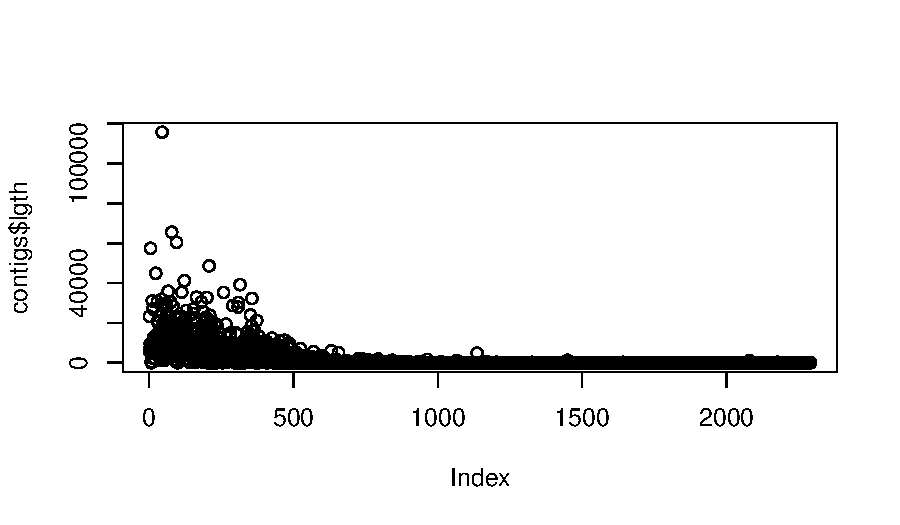
\includegraphics{plots/figura-024}
\end{frame}

\subsection{Líneas}

\begin{frame}[fragile, allowframebreaks]
  \frametitle{Lines}
  \scriptsize 
\begin{Schunk}
\begin{Sinput}
> plot(log10(sort(contigs$lgth)), 
+     type = "l")
> lines(log10(1:length(contigs$lgth)^2), 
+     col = "red")
\end{Sinput}
\end{Schunk}
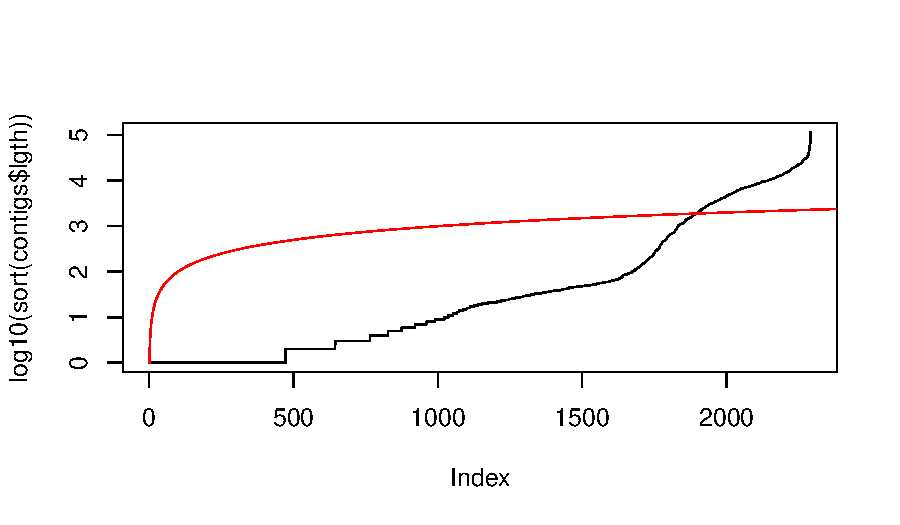
\includegraphics{plots/figura-025}
\normalsize
\end{frame}

\subsection{Gráfica de barras}

\begin{frame}[fragile, allowframebreaks]
  \frametitle{Barplot}
  \scriptsize 
\begin{Schunk}
\begin{Sinput}
> barplot(contigs$lgth[contigs$lgth > 
+     30000]/1000, col = rainbow(length(contigs$lgth[contigs$lgth > 
+     30000])), xlab = "Contigs larger than 30kb", 
+     ylab = "Length in kb", main = "Largest contigs")
\end{Sinput}
\end{Schunk}
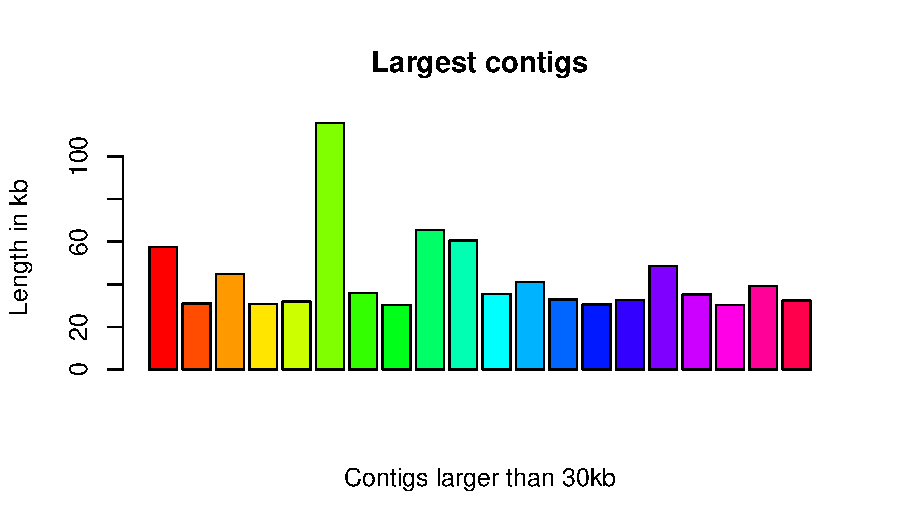
\includegraphics{plots/figura-026}
\normalsize
\end{frame}

\subsection{Histograma}

\begin{frame}[fragile, allowframebreaks]
  \frametitle{Histograma básico}
\begin{Schunk}
\begin{Sinput}
> hist(contigs$lgth, col = "lightblue")
\end{Sinput}
\end{Schunk}
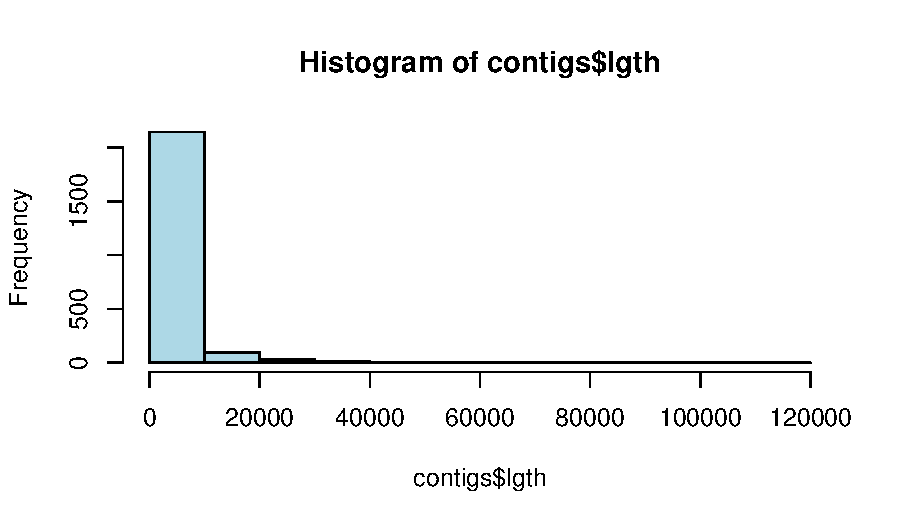
\includegraphics{plots/figura-027}
\end{frame}

\subsection{Densidad}

\begin{frame}[fragile, allowframebreaks]
  \frametitle{Graficando la densidad}
\begin{Schunk}
\begin{Sinput}
> hist(contigs$lgth, col = "lightblue", 
+     prob = T)
> lines(density(contigs$lgth), col = "red")
\end{Sinput}
\end{Schunk}
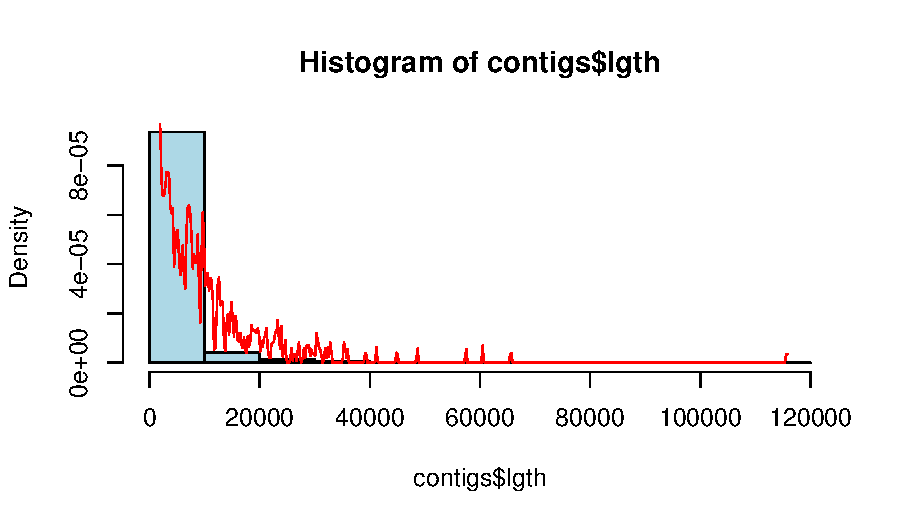
\includegraphics{plots/figura-028}
\end{frame}

\subsection{Diagrama de caja y brazos}

\begin{frame}[fragile, allowframebreaks]
  \frametitle{Resumen gráfico}
\begin{Schunk}
\begin{Sinput}
> boxplot(contigs$lgth, rnorm(1000, 
+     40000, 10000), col = c("lightblue", 
+     "red"))
\end{Sinput}
\end{Schunk}
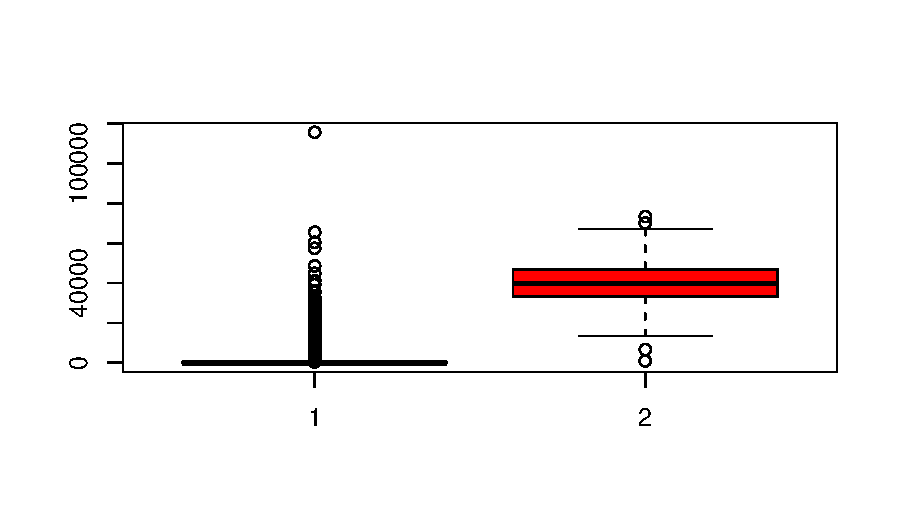
\includegraphics{plots/figura-029}
\end{frame}


\subsection{Mosaicplot}

\begin{frame}[fragile, allowframebreaks]
  \frametitle{Excelente para tablas con 3 dims}
\begin{Schunk}
\begin{Sinput}
> mosaicplot(HairEyeColor, shade = TRUE)
\end{Sinput}
\end{Schunk}
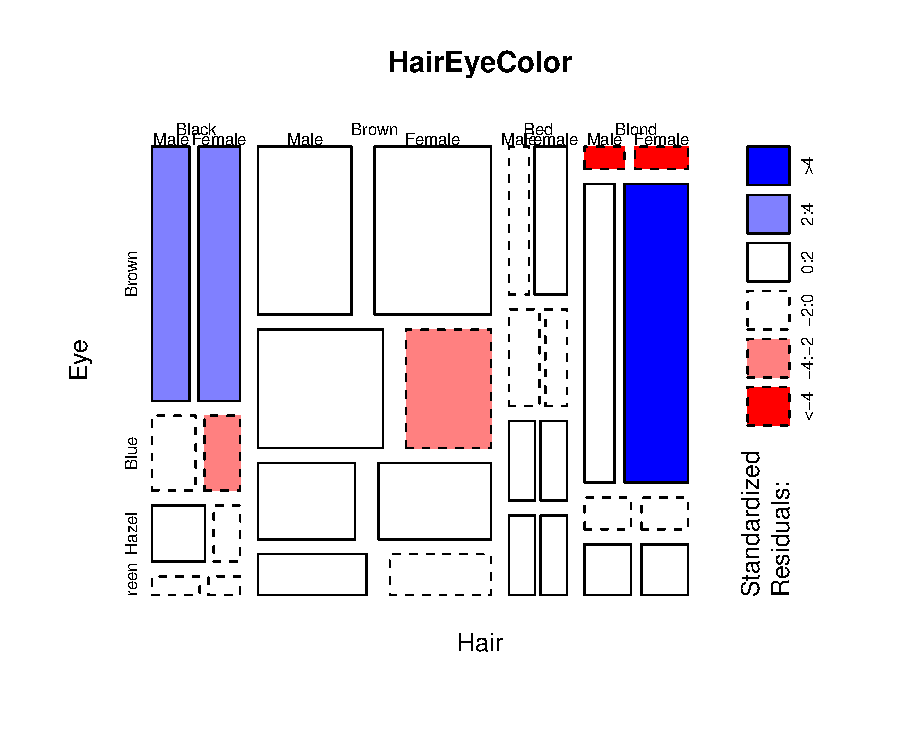
\includegraphics{plots/figura-030}
\end{frame}

\subsection{Imagen}

\begin{frame}[fragile, allowframebreaks]
  \frametitle{Te ayuda a visualizar tu matriz}
\begin{Schunk}
\begin{Sinput}
> x <- matrix(1:100, 10, 10, byrow = T)
> image(x, col = heat.colors(100))
\end{Sinput}
\end{Schunk}
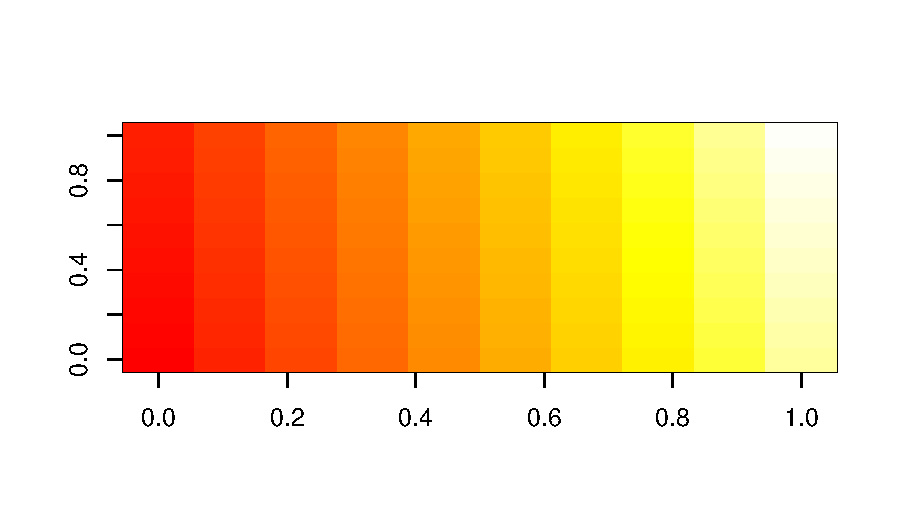
\includegraphics{plots/figura-031}
\end{frame}

\subsection{PDF y PNG}

\begin{frame}[allowframebreaks, fragile]
  \frametitle{Exportando im\'agenes}
  \begin{itemize}
  \item Siempre puedes exportar tus im\'agenes a archivos PDF o PNG.
\begin{Schunk}
\begin{Sinput}
> pdf(file = "file.pdf", onefile = T)
> plot("some data")
> dev.off()
> png(file = "image.png")
> plot("some data")
> dev.off()
\end{Sinput}
\end{Schunk}
  \end{itemize}
\end{frame}


%%%%%%%%%%%%%%%%%%%%%%%%%%%%%%%%%%%%%%%%%%%%%%%%%%%%%%%%%%%%%%%%%%%%%%%%%%%
\section{Control de flujo}

\begin{frame}[allowframebreaks, fragile]
  \frametitle{Dos opciones}
  \begin{itemize}
  \item \BIOCfunction{While} es muy f\'acil de usar: \pl{while (cond) expr}
\begin{Schunk}
\begin{Sinput}
> x <- NULL
> while (length(x) < 10) {
+     x <- c(x, runif(1))
+ }
\end{Sinput}
\end{Schunk}
  \item \textquestiondown Cu\'al es la longitud del objeto \pl{x}? Ahora usemos \BIOCfunction{repeat} con \BIOCfunction{break}.
  \item Con \pl{while} y \pl{repeat} se cuidadoso y evita \alert{ciclos infinitos!}
\begin{Schunk}
\begin{Sinput}
> x <- 1
> repeat {
+     x <- x + 2
+     print(x)
+     if (x > 10) 
+         break
+ }
\end{Sinput}
\begin{Soutput}
[1] 3
[1] 5
[1] 7
[1] 9
[1] 11
\end{Soutput}
\end{Schunk}
  \end{itemize}
\end{frame}

\begin{frame}[allowframebreaks, fragile]
  \frametitle{Una alternativa}
  \begin{itemize}
  \item La forma m\'as com\'un de iteraci\'on es un ciclo \alert{for}: \pl{for (var in seq) expr}
\begin{Schunk}
\begin{Sinput}
> for (i in seq_len(3)) print(i)
\end{Sinput}
\begin{Soutput}
[1] 1
[1] 2
[1] 3
\end{Soutput}
\begin{Sinput}
> for (i in letters[4:6]) print(i)
\end{Sinput}
\begin{Soutput}
[1] "d"
[1] "e"
[1] "f"
\end{Soutput}
\end{Schunk}
  \item Usar \pl{seq\_len} es lo m\'as recomendado en vez de usar \pl{1:length(object)}
  \item Como querr\'as usar condiciones \BIOCfunction{if}, \BIOCfunction{ifelse} y \BIOCfunction{switch} ser\'an de tu inter\'es.
  \end{itemize}
\end{frame}

\subsection{Creando funciones}

\begin{frame}[allowframebreaks, fragile]
  \frametitle{Bases}
  \begin{itemize}
  \item Es muy f\'acil escribir tus propias funciones de \pl{R} usando \BIOCfunction{function}.
  \item As\'i como puede aceptar muchos argumentos de entrada, s\'olo regresa \alert{un} objeto que puede ser un vector.
  \item El objeto que se regresa es o el \'ultimo en ser evaluado o alguno especificado con la funci\'on \BIOCfunction{return}. 
  \item Si se usa un objeto x dentro de la funci\'on, \'este no estar\'a relacionado con la variable x fuera de la funci\'on .\footnote{Los usuarios m\'as curiosos pueden buscar gu\'ias acerca de los ambientes}
\begin{Schunk}
\begin{Sinput}
> x <- 5
> y <- function(x) rnorm(x)
> y(2)
\end{Sinput}
\begin{Soutput}
[1]  0.3796838 -0.8461351
\end{Soutput}
\begin{Sinput}
> x
\end{Sinput}
\begin{Soutput}
[1] 5
\end{Soutput}
\end{Schunk}
  \end{itemize}
\end{frame}

\subsection{Funciones Apply}

\begin{frame}[allowframebreaks, fragile]
  \frametitle{Una familia ejemplar}
  \begin{itemize}
  \item Su mayor utilidad es \emph{aplicar} una funci\'on a todos los elementos de un objeto. Por ejemplo, todos los elementos de una matriz.
  \item En muchos de los casos, es simplificado o en algunos otros es un argumento.
  \item Es m\'as facil para una persona entender un script con funciones \BIOCfunction{apply} que con ciclos \pl{for}.
\begin{Schunk}
\begin{Sinput}
> mat <- matrix(rnorm(100), 10, 10)
> apply(mat, 1, sum)
\end{Sinput}
\begin{Soutput}
 [1]  2.241366 -3.799676  2.924169
 [4]  0.905126  7.618892  2.001233
 [7] -6.468566 -3.374802 -3.162069
[10] -3.786084
\end{Soutput}
\end{Schunk}
  \item Recuerda que algunas funciones de \pl{R} son m\'as r\'apidas usando apply, como \BIOCfunction{rowMeans}.
\begin{Schunk}
\begin{Sinput}
> apply(mat, 1, sum) == rowSums(mat)
\end{Sinput}
\begin{Soutput}
 [1] TRUE TRUE TRUE TRUE TRUE TRUE TRUE
 [8] TRUE TRUE TRUE
\end{Soutput}
\end{Schunk}
  \item Algunos paquetes implementan nuevas funciones \pl{apply} pero las m\'as comunes son:
  \begin{itemize}
  \item \pl{apply} \'util para matrices y data frames
  \item \pl{lapply} La versi\'on para listas
  \item \pl{sapply} La m\'as sencilla (listas y vectores).
\begin{Schunk}
\begin{Sinput}
> x <- list(rnorm(100), runif(100), 
+     rlnorm(100))
> sapply(x, quantile)
\end{Sinput}
\begin{Soutput}
            [,1]       [,2]       [,3]
0%   -2.42221515 0.03082297  0.1807016
25%  -0.58079951 0.26005973  0.5831613
50%  -0.01462831 0.47147562  1.1230483
75%   0.77904047 0.70181975  2.2492986
100%  2.59119996 0.98880743 12.9508204
\end{Soutput}
\end{Schunk}
  \item \pl{tapply} Usa un vector y un factor, muy \'util para datos agrupados.
\begin{Schunk}
\begin{Sinput}
> x <- data.frame(info = rnorm(10), 
+     group = as.factor(sample(1:3, 
+         10, replace = T)))
> tapply(x$info, x$group, mean)
\end{Sinput}
\begin{Soutput}
         1          2          3 
 0.2763497 -0.8849198  0.5146212 
\end{Soutput}
\end{Schunk}
  \item \pl{eapply} Para ambientes y los curiosos.
  \item \pl{mapply} Versi\'on multivariada de \pl{sapply}
\begin{Schunk}
\begin{Sinput}
> mapply(rep, 1:4, 4:1)
\end{Sinput}
\begin{Soutput}
[[1]]
[1] 1 1 1 1

[[2]]
[1] 2 2 2

[[3]]
[1] 3 3

[[4]]
[1] 4
\end{Soutput}
\end{Schunk}
  \item \pl{rapply} Versi\'on recursiva de \pl{lapply}
  \end{itemize}
  \item Este sitio puede parecerte \'util: \myurlshort{www.ats.ucla.edu/stat/r/library/advanced\_function\_r.htm}{advanced\_function\_r.htm}
  \end{itemize}
\end{frame}

%%%%%%%%%%%%%%%%%%%%%%%%%%%%%%%%%%%%%%%%%%%%%%%%%%%%%%%%%%%%%%%%%%%%%%%%%%%
\section{Ejercicios}

\begin{frame}[allowframebreaks]
  \frametitle{o tarea :P}
  \begin{itemize}
  \item Ve al \myurlshort{www.lcg.unam.mx/~lcollado/B/}{sitio oficial del curso} y realiza el primer ejercicio.
  \item Las especificaciones de la tarea est\'an en el \pl{syllabus}. 
  \begin{itemize}
    \item Para esta tarea s\'olo entrega un script portable \pl{.R} con comentarios. La siguiente semana aprenderemos acerca de los archivos \pl{Sweave} y \emph{vignette}.
  \end{itemize}
  \end{itemize}
\end{frame}


\end{document}
